		\item{\bf Solar Physics}\\
		\begin{enumerate}
			%
			\item{\em Basic Information about the Sun \citep[see][]{carroll_introduction_2007}}
			\begin{enumerate}
				\item{Radiative interior}
				\par Radiation allows the energy produced by nuclear reactions and gravitation to be carried to the surface via photons, where the photons undergo a ``random walk'' as they make their way from the core to the surface. This overall motion toward the surface is due to the fact that $dT/dr<0$. This decrease in temperature causes a decrease in radiation pressure with increasing $r$, leading to a ``photon breeze'' that carries the radiative flux towards the surface. This is accomplished through the slow upward diffusion of photons to the surface. Typically, radiation is the dominant transport process deep in the core and gives way to convection as $r$ increases and the temperature gradient steepens.
				\item{Convective envelope}
				\par Convection can be a very efficient transport mechanism. Hot, buoyant mass elements carry excess energy outward while cool mass elements fall inward. Convection is the dominant transport process in the outer layer of the Sun and is the dominant process over radiation once the temperature gradient has steepened appreciably, in particular $\left|dT/dr\right|>\left|dT/dr\right|_{ad}$, that is, if the temperature gradient is ``super adiabatic''. 
				\item{Radius}
				\par The radius of the sun is $R_{\odot} = 6.95508\times10^8$ m.
				\item{Mass}
				\par The mass of the Sun is $M_{\odot} = 1.9891\times10^{30}$ kg.
				\item{Luminosity}
				\par The effective luminosity of the Sun is $L_{\odot} = 3.839\times10^5$ W.
				\item{Structure of atmosphere}
				%
				\par Though the Sun can be easily seen from Earth, its dynamic and highly structured atmosphere is not observable with the naked eye, with the one exception being brief glimpses of the corona during an eclipse. The interior of the Sun is of course very complex and constitutes a very different regime of physics than that seen in the solar atmosphere. Thus, this work will be primarily limited to the upper solar atmosphere with some discussion of the lower layers.
				%
				\par The solar atmosphere is often divided up into four separate regions: the photosphere, the chromosphere, the transition region, and the corona. Fig. \ref{fig:cartoon_layers} shows a cartoon of the different layers while Fig. \ref{fig:graph_layers} shows the density and temperature profiles of the atmosphere with each region labeled. The \textit{photosphere} is what we typically refer to as the solar surface, with the actual surface located where the optical depth, $\tau$, is equal to 1. This region also contains the lowest temperature on the Sun, approximately 4400 K, located about 525 km above the surface \citep{carroll_introduction_2007}. The photosphere is where the majority of the visibly (with the naked eye) observable photons originate.
				%
				\par The temperature minimum defines the top of the photosphere above which lies the \textit{chromosphere}. As can be seen from Fig. \ref{fig:graph_layers}, the density in the chromosphere is many orders of magnitude less than that of the photosphere and the temperature has increased from the minimum up to about $1\times10^4$ K. Though not visible with the naked eye, the chromosphere is highly structured. Structures such as spicules, tall columns of gas that extend high into the solar atmosphere thought to heavily impact the behavior of plasma in the corona \citep{de_pontieu_origins_2011}, originate in the photosphere as well as filaments, essentially spicules observed on-disk and plage, bright regions surrounding sunspots.
				%
				\begin{figure}[htbp]
					\centering
					\subfigure[]{%
					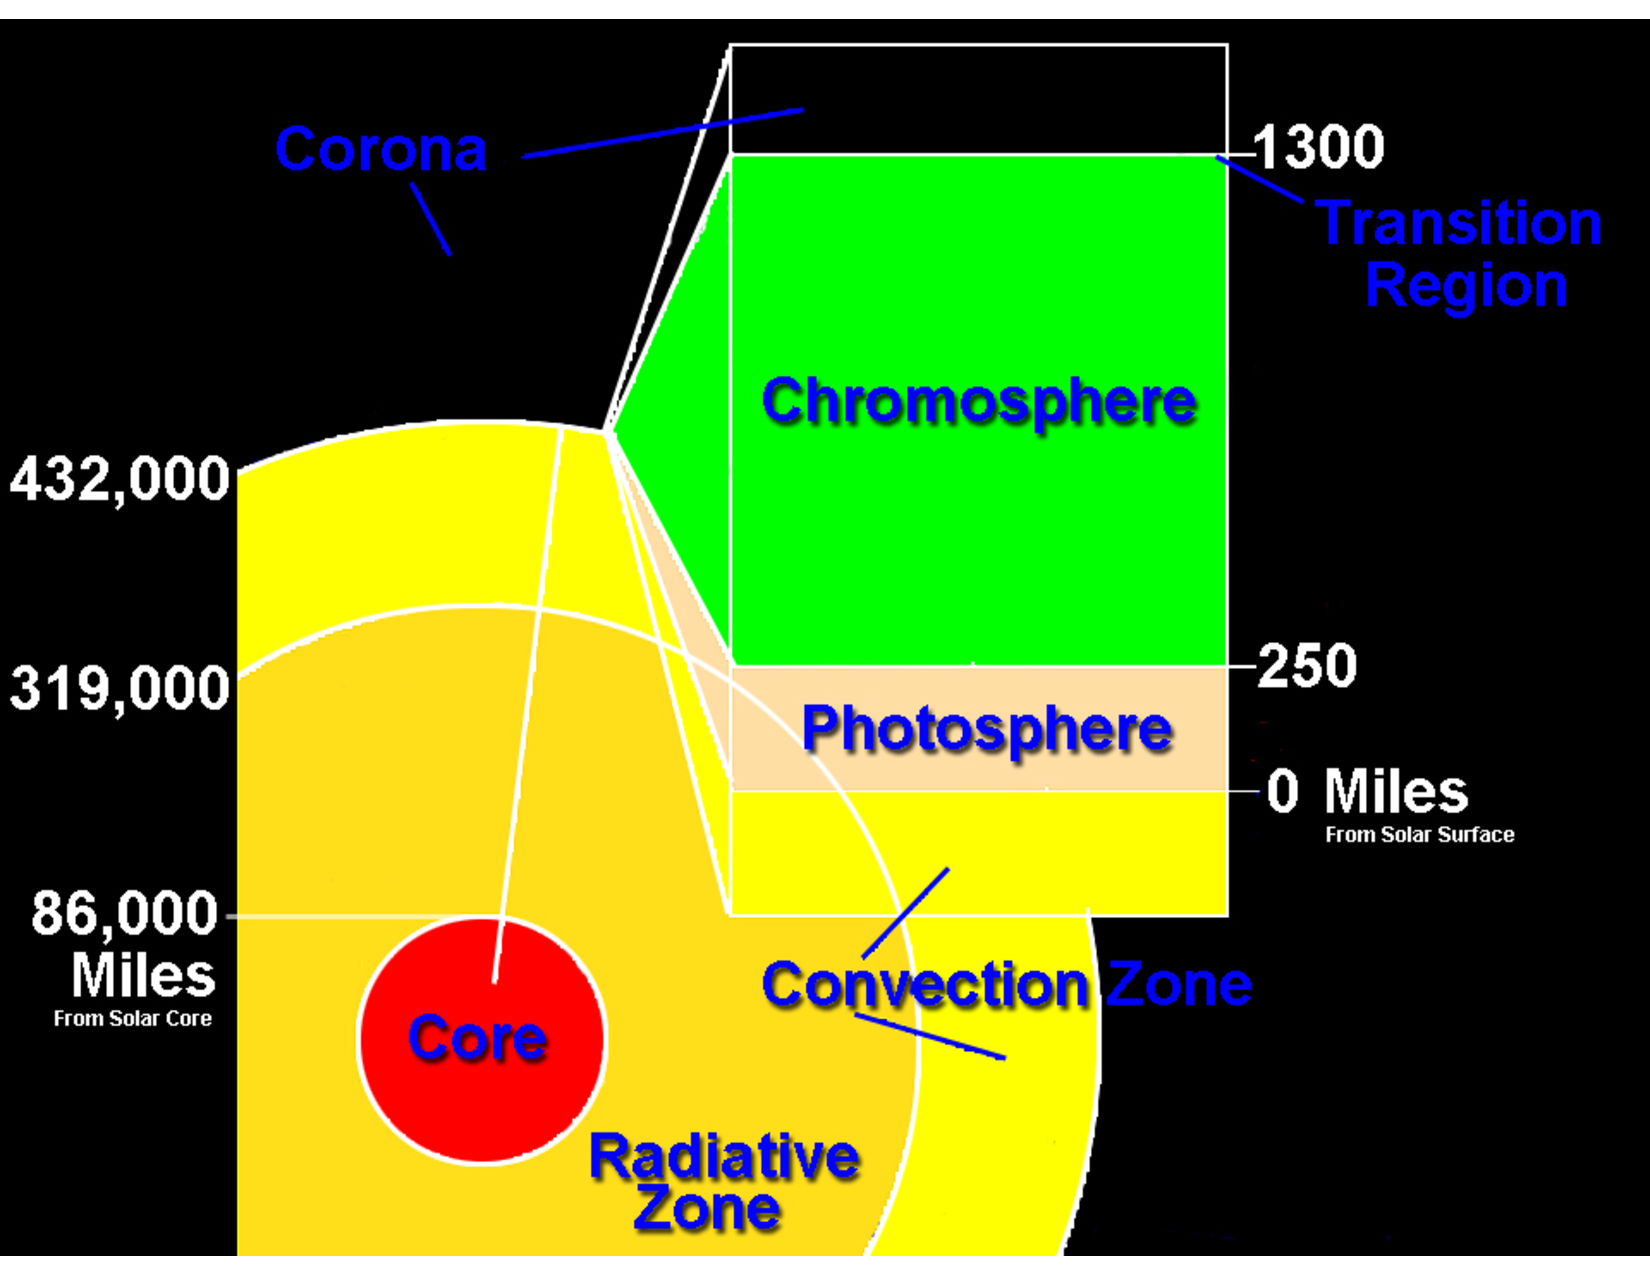
\includegraphics[width=0.45\textwidth]{figures/cartoon_layers.pdf}
					\label{fig:cartoon_layers}}
					\subfigure[]{%
					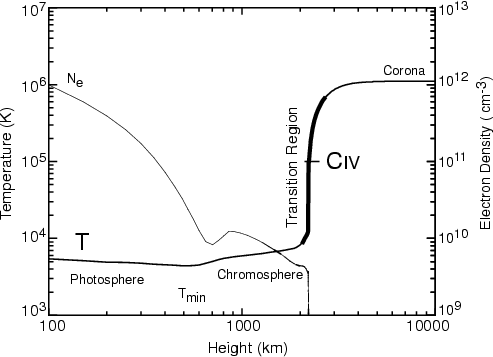
\includegraphics[width=0.45\textwidth]{figures/diagram_layers.png}
					\label{fig:graph_layers}}
					\caption{\textbf{(a)} Schematic showing the layers of the solar atmosphere; the corona is the uppermost layer of the atmosphere. Courtesy of NASA \textbf{(b)} Temperature and density as a function of height above the solar surface; the corona is characterized by low densities and anomalously-high temperatures. Taken from \citet{gary_solar_2007}}
					\label{fig:layers}
				\end{figure} 
				%
				\par Next is the \textit{transition region}, so called because of the steep temperature and density gradients (see Fig. \ref{fig:graph_layers}) that mark the transition between the chromosphere and the corona. The transition region is extremely thin, only a few hundred kilometers as compared to the chromosphere which extends over many thousands of kilometers. However, in this very short change in altitude, the temperature in the solar atmosphere jumps from $\approx1\times10^4$ K to temperatures exceeding $1\times10^5$ K. 
				%
				\par Finally, the solar \textit{corona}, or ``crown'', is the highly-dynamic uppermost layer of the Sun's atmosphere. Visible with the naked eye only during a total solar eclipse, the corona is highly-structured and diffuse. Here, the temperature continues to increase, with typical coronal temperatures exceeding $1\times10^6$ K. Particularly high temperatures ($\approx1\times10^7$ K) have also been observed in \textit{active regions}, sites of intense magnetic activity associated with sunspots. These active regions can contain plasma as cool as $1\times10^4$ K as well and represent some of the most dynamic portions of the solar corona.
				%
				\item{Additional Typical Parameters}
				\begin{itemize}
					\item $B$-field strength in Active Region: $\sim10^3$ G
					\item $B$-field strength in quiet sun: $\sim10$ G
					\item For typical coronal parameters, $\kappa_{\parallel}/\kappa_{\perp}\gg10^{8}$, where $\kappa$ is the thermal conductivity. This explains why energy transported by thermal conduction travels almost exclusively in the field-aligned direction. Cross-field transport by thermal conduction is negligible. 
					\item $\beta\equiv p/(B^28\pi)\ll1$ in the corona. This also explains confinement of coronal plasma. The corona is considered a ``low-$\beta$'' plasma.
					\item The mean free path in the corona can be estimated as,
					\begin{equation}
						\ell_{mfp}=v\tau\approx \frac{v_{th}}{\nu_{ee}}\approx 4.67\times10^{7}\left(\frac{T}{10^6~\mathrm{K}}\right)^2\left(\frac{n}{10^8~\mathrm{cm}^{-3}}\right)^{-1}~\mathrm{cm}.
					\end{equation}
					Thus, for $T\sim1$ MK and $n\sim10^8~\mathrm{cm}^{-3}$, $\ell_{mfp}\sim500$ km. 
				\end{itemize}
			\end{enumerate}
			%
			\item{\em Radiative Transfer}
			\begin{enumerate}
				\item{Specific intensity}
				\par The specific intensity, or brightness, $I_{\nu}$, is defined by the equation
				\begin{equation}
					\label{eq:spec_intensity}
					dE=I_{\nu}dAdtd\Omega d\nu,
				\end{equation}
				where $dE$ is the energy crossing $dA$ in time $dt$ in frequency range $d\nu$. 
				\item{Limb darkening}
				\par Limb darkening is the effect of the apparent brightness of an object decreasing as you move away from the center. As seen in Fig. \ref{fig:limb_darkening}, as we move away from the center of the object, the angle $\theta$ between the LOS and the vector pointing radially outward from the center increases. Recall that $\tau_{\nu}$ can be thought of as the number of mean free paths it takes to get from the source to the surface and that observed photons from Sun-like stars originate from an optical depth of $\sim2/3$. 
				\par We can define a maximum penetration depth (or origin depth, more precisely) as $d=2/3\ell$, where $\ell$ is the mean free path. When $\theta=0$, the radius from which the observed photon originates is equal to $d$. As $\theta$ increases, the depth of origin increases, meaning the observed intensity comes from greater and greater radii. Starting at the photosphere and going toward the core, temperature increases with radii such that intensity from lesser radii correspond to hotter plasma. To a first approximation, the Sun can be treated as a blackbody, meaning for a given $\lambda$, intensity increases with temperature. Thus, intensity coming from deeper inside the Sun (and consequently lesser radii) corresponds to brighter intensity. 
				\begin{figure}
					\centering
					\includegraphics[width=0.5\textwidth]{figures/limb_darkening.pdf}
					\caption{Limb darkening schematic taken from \citet[Ch. 9]{carroll_introduction_2007}.}
					\label{fig:limb_darkening}
				\end{figure}
				%
				\item{Transfer equation}
				\par The specific intensity is constant along rays in free space such that 
				\begin{equation}
					\frac{dI_{\nu}}{ds}=0.
				\end{equation}
				However, if rays pass through matter, energy may be added through emission or absorption processes. In the case of emission, we define an emission coefficient $j_{\nu}$ as the energy emitted per unit time per unit solid angle per unit volume per unit frequency,
				\begin{equation}
					dE=j_{\nu}dVd\Omega dtd\nu.
				\end{equation}
				From Eq. \ref{eq:spec_intensity}, we can define the emission term as 
				\begin{equation}
					\frac{dI_{\nu}}{ds} = j_{\nu},
				\end{equation}
				where $j_{\nu}ds$ represents intensity added to the beam by spontaneous emission. Conversely, we can define an absorption coefficient $\alpha_{\nu}$ as 
				\begin{equation}
					\frac{dI_{\nu}}{ds} = -\alpha_{\nu}I_{\nu}.
				\end{equation}
				For a collection of particles with density $n$ and cross-section $\sigma_{\nu}$, the effective absorption area is $ndAds\sigma_{\nu}$. Thus, using Eq. \ref{eq:spec_intensity}, $\alpha_{\nu} = n\sigma_{\nu}$. Often, $\alpha_{\nu}$ is expressed as $\alpha_{\nu}=\rho\kappa_{\nu}$, where $\rho$ is the mass density and $\kappa_{\nu}$ is called the mass absorption or opacity coefficient. 
				\par The total radiative transfer equation is thus defined as 
				\begin{empheq}[box=\widefbox]{align}
					\label{eq:transfer}
					\frac{dI_{\nu}}{ds} = j_{\nu} - \alpha_{\nu}I_{\nu}.
				\end{empheq}
				To make things a bit easier, we can define the \textit{optical depth} as $d\tau_{\nu}=\alpha_{\nu}ds$. When $\tau_{\nu}>1$, the medium is said to be optically thick; when $\tau_{\nu}<1$, the medium is said to be optically thin or transparent. In an optically thin medium, a photon of frequency $\nu$ can traverse the medium without being absorbed. Note: the optical depth may be thought of as the number of mean free paths from the original position to the surface, as measured along the ray's path \citep{carroll_introduction_2007}.
				\par Next we define the source function $S_{\nu}=j_{\nu}/\alpha_{\nu}$ as well as the variables $\mathcal{J}\equiv I_{\nu}e^{\tau_{\nu}}$ and $\mathcal{S}\equiv S_{\nu}e^{\tau_{\nu}}$, we can rewrite the transfer equation as 
				\begin{equation}
					\frac{d\mathcal{J}}{d\tau_{\nu}}=\mathcal{S}.
				\end{equation}
				Using this equation and substituing back in $I_\nu$, we can write the formal solution of the transfer equation as
				\begin{empheq}[box=\widefbox]{align}
					\label{eq:transfer_soltn}
					I_{\nu}(\tau_{\nu}) = I_{\nu}(0)e^{-\tau_{\nu}} + \int_0^{\tau_{\nu}}\mathrm{d}\tau'_{\nu}~e^{-(\tau_{\nu} - \tau'_{\nu})}S_{\nu}(\tau'_{\nu}).
				\end{empheq}
				We note that this equation is the sum of two terms: (1)the initial intensity diminished by absorption and (2) the integrated source diminished by absorption.
				\par Additionally, we can define the \textit{mean free path} as the average distance a photon can travel through an absorbing material without being absorbed. For a homogenous material, the mean optical depth, $\langle\tau_{\nu}\rangle=1$. The mean free path, $\ell_{\nu}$ can be written as $\langle\tau_{\nu}\rangle=\ell_{\nu}\alpha_{\nu}$ such that $\ell_{\nu}=1/\alpha_{\nu}$. Note that $\ell_{\nu}$ is inversely proportional to both density, $n$, and cross-section, $\sigma_{\nu}$.
			\end{enumerate}
			%
			\item{\em Hydrostatic Atmospheres}
			\begin{enumerate}
				\item{Hydrostatic equilibrium}\\
				\par Because $\beta\ll1$ and observations have shown that coronal loop structures are relatively long-lived (on the timescale of hours or even days), coronal plasma can be modeled in terms of the fundamental loop structure, where all motion is constrained to be in the field-aligned direction. Provided the magnetic field is changing on slow timescales relative to the plasma dynamics, $B$ only plays the role of confining the plasma and does not alter its dynamics.
				\par A reasonable assumption in the corona, particular in the period where temporal resolution of coronal observations was comparatively poor, is that of hydrostatic equilibrium, where the energy input into the corona is balanced by redistribution by thermal conduction and losses to space by radiation such that,
				\begin{empheq}[box=\widefbox]{align}
					\label{eq:hydrostatic_energy}
					E_H - \frac{d}{ds}F_C - E_R = 0,
				\end{empheq}
				where $E_H$ is the \textit{ad-hoc} heating input into the corona, $E_R=n^2\Lambda(T)$ is the volumetric radiative loss where $\Lambda(T)$ is the power-law radiative loss function, and $F_C=-\kappa_0T^{5/2}dT/ds$ is the heat flux as given by the classical Spitzer formula, with $\kappa_0\approx10^{-6}$. 
				\par The pressure balance is maintained between the downward graviational pressure and the counter-acting thermal pressure such that 
				\begin{empheq}[box=\widefbox]{align}
					\frac{d}{ds}p = -\rho g_{\parallel},
				\end{empheq}
				where $\rho$ is the mass density and $g_{\parallel}$ is the gravitational acceleration parallel to the field aligned direction. Furthermore, these equations are all closed by the equation of state,
				\begin{equation}
					p=2nk_BT,
				\end{equation}
				the ideal gas law. Note that in the isothermal case, $dF_C/ds=0$ and we can solve the energy and pressure balance equations analytically. For a straight, gravitationally-stratified loop, the pressure can be expressed as $p=p_0\exp{-h/S_p},$ the density as $n=n_0\exp{-h/S_p},$ and the heating rate as $E_H=n_0^2\Lambda(T)\exp{-h/S_H},$ where $S_H=S_p/2$ is the heating scale height, $S_p=\lambda_p(1+h/R_0)$ is the pressure scale height, and $\lambda_p=2k_BT/m_ig_0$ is the hydrostatic scale height. Note that this implies that low-temperature emission is likely to be confined near the footpoints (because $n$ drops off rapidly with $h$) while high-temperature emission is more likely to be found at higher altitudes. 
				\par For non-isothermal solutions, we must often resort to numerical solutions. We can rewrite the energy balance equation such that $dF_C/ds=E_H-E_R$. Thus, when $E_H<E_R$, the heat flux must make up for the deficit in the heating relative to the radiative losses while in the case that $E_H>E_R$, the heat flux must carry off excess heat that can't be gotten rid of through only radiative losses.
				\item{Coronal heating scaling laws}\\
				\citep[see][]{rosner_dynamics_1978,martens_scaling_2010}
				\par The scalings laws can be derived using the hydrostatic energy balance equation, Eq. \ref{eq:hydrostatic_energy}. By making an isobaric (i.e. $p=\mathrm{constant}$), the equation becomes separable in $F_C$ and $T$ such that,
				\begin{equation}
					F_C^2(T) = f_R(T) - f_H(T),
				\end{equation}
				where $f_R,f_H$ are $T$-integrals over the radiation and heat terms, respectively. Because we know the form of $F_C(T)$, we note that the above equation is separable in $s$ and $T$ such that
				\begin{equation}
					\label{eq:scaling_starting}
					s(T) - s(T_0) = \kappa_0\int_{T_0}^T\mathrm{d}\mathcal{T}~\mathcal{T}^{5/2}(f_R(\mathcal{T}) - f_H(\mathcal{T}))^{-1/2},
				\end{equation}
				where $T_0$ is the coronal base temperature. Note that since $\Lambda(T)$ can be approximated by a power-law, $\Lambda=\chi T^{\alpha},$ and for $T>10^5$ K, $\alpha=-1/2,~\chi=10^{-18.8}$, $f_R(T)\propto T$. 
				\par To derive the first scaling law, we consider the case at the base of the loop where $f_R\gg f_H$. Using the approximation $T_0\ll T_{max}$, we find the first scaling law relating the maximum temperature, pressure, and loop length,
				\begin{empheq}[box=\widefbox]{align}
					\label{eq:rtv_scaling_1}
					T_{max} = C_1(pL)^{1/3},
				\end{empheq}
				where $C_1=(3/\kappa_0)^{1/3}(\kappa_0\chi/2k_B^2)^{1/6}\approx1.83\times10^3$ is the constant of proportionality. 
				\par To derive the second scaling law, consider the case at the apex of the loop. For uniform heating, $F_C(T_{a})=0$ such that $f_R(T)=f_H(T)$.  Integrating on $T_0\le T\le T_{max}$ and using the approximation $T_0\ll T_{max}$, we find that $E_H\propto T_{max}^{-5/2}p^2$. Using the first scaling law, Eq. \ref{eq:rtv_scaling_1}, we can easily find that
				\begin{empheq}[box=\widefbox]{align}
					\label{eq:rtv_scaling_2}
					E_H = C_2p^{7/6}L^{-5/6},
				\end{empheq}
				where $C_2=5.09\times10^4$. 
				%
				\par Note that \citet{rosner_dynamics_1978} derived these scaling laws for x-ray (through the choice of $f_R$) loops and assumed maximum temperature at the apex as well as spatially-uniform heating and pressure. While these laws generally agree with x-ray observations, they do not match up well with EUV loop observations. For example, EUV loops have been observed to be overdense relative to x-ray loops, indicating that they cannot be adequately described by hydrostatic equilibrium.  
				%
				\item{Additional Notes on Hydrostatic results}
				\begin{itemize}
					\item Revised scaling laws by \citet{serio_closed_1981} were derived to correct for varying pressure and non-uniform heating. Factors of $\exp{(-0.04L(2/S_H-1/S_p))}$ and $\exp{(0.5L(1/S_H-1/S_p))}$ are added to Eq. \ref{eq:rtv_scaling_1} and Eq. \ref{eq:rtv_scaling_2}, respectively. 
					\item Thermal conduction is an energy sink ($-dF_C/ds<0$) in the corona and an energy source ($-dF_C/ds>0$) in the transition region such that the point at which $dF_C/ds=0$ provides a convenient way to define the interface between the two distinct regions.
					\item Using the fact that $E_H=E_R$ at the boundary along the scaling laws, it can be shown that $T_0=0.6T_{max}.$
					\item Thus, the corona and transition region are not simply separated by different temperature ranges, but rather by fundamental differences in the energy balance.
				\end{itemize}
				%
			\end{enumerate}
			%
			\item{\em Magnetic Field}
			\begin{enumerate}
				\item{Potential versus force-free}\\
				\citep[see][]{aschwanden_physics_2006}
				%
				\par\textbf{Potential:} When a force field can be expressed as $\mathbf{F}(\mathbf{r})=\nabla\phi(\mathbf{r})$, we call $\mathbf{F}(\mathbf{r})$ a potential field. In the same way, we can define a magnetic potential field by
				\begin{equation}
					\label{eq:potential field}
					\mathbf{B}(\mathbf{r}) = \nabla\phi(\mathbf{r}),
				\end{equation}
				where $\phi$ is the magnetic scalar potential function. Because Maxwell's equations demand that $\nabla\cdot\mathbf{B}=0$, the scalar potential satisfies Laplace's equation $\nabla^2\phi=0$. Recalling that $\mathbf{j}=(1/4\pi)\nabla\times\mathbf{B}$, substituting in our potential field expression yields $\mathbf{j}=0$. Thus, a magnetic potential field is equivalent to a ``current-free'' field. Two easy ways to describe these fields are through either a dipolar or unipolar approach. 
				\par The only way to ``measure'' the solar magnetic field is through Zeeman splitting via magnetograms, measurements of the field strength at the photosphere. Thus, the coronal field must be inferred from these values at the photospheric boundary (i.e. a boundary problem) via some field extrapolation method. This essentially boils down to solving Laplace's equation for an assumed set of boundary conditions. Two popular methods for doing this are either through Green's function methods or through eigenfunction expansions. Using the method of \citet{sakurai_greens_1982}, a Green's function method is used to perform the extrapolation using boundary conditions at $r=a,$ the photospheric surface values known from magnetograms and at $r=b$, the so-called source surface at which the field is assumed to be only radial and connect with the solar wind.
				%
				\par\textbf{Force-free:} Using the Lorentz force, $n$ particles each with charge $q$ and moving with velocity $\mathbf{v}$ in a magnetic field $\mathbf{B}$ are subject to a force $\mathbf{F}=(q/c)n(\mathbf{v}\times\mathbf{B})$. Because $\mathbf{j}=(q/c)n\mathbf{v}$, the Lorentz force in MHD is generally written as $\mathbf{F}=\mathbf{j}\times\mathbf{B}$. In magneto-statics, a magnetic field is said to be force-free when the ``self-force'' is zero or in this case, $\mathbf{j}\times\mathbf{B}=0$. Using the definition $\mathbf{j}=(1/4\pi)\nabla\times\mathbf{B}$, the force-free condition can be rewritten as 
				\begin{equation}
					\label{eq:force_free_field}
					(\nabla\times\mathbf{B})\times\mathbf{B} = 0.
				\end{equation}
				Note that in general this is a non-trivial calculation since it involves non-linear terms of order $B^2$.
				\par Two different cases of force-free fields are usually considered: linear and non-linear. Consider $\nabla\times\mathbf{B}=\alpha(\mathbf{r})\mathbf{B}$, where $\alpha(\mathbf{r})$ is some scalar function. Note that $\alpha\neq0$ implies a non-potential field while $\alpha=0$ corresponds to the potential field case. We require $\mathbf{B}$ to satisfy the condition  $\nabla\cdot\mathbf{B}=\nabla\cdot(\nabla\times\mathbf{B})=0\rightarrow\mathbf{B}\cdot\nabla\alpha=0$. Thus, when we plug in our general form to our force-free requirement, Eq. \ref{eq:force_free_field}, we have the equations we need to satisfy,
				\begin{align}
					\nabla^2\mathbf{B}+\alpha^2\mathbf{B} &= \mathbf{B}\times\nabla\alpha(\mathbf{r}), \\
					\mathbf{B}\cdot\nabla\alpha(\mathbf{r}) &= 0.
				\end{align}
				When $\alpha=\mathrm{constant}$, we are left with the Helmholtz equation. This is usually referred to as the linear (lfff) case. Otherwise, if $\alpha(\mathbf{r})$ is a general function of position, we have the non-linear (nlfff) case.
				%
				\item{Open versus closed}
				\par ``Open'' field lines are those field lines who have one end rooted in the solar surface and the other end connecting to the interplanetary magnetic field/solar wind. Closed magnetic field lines have both ends rooted in the solar surface. In both cases $\nabla\cdot\mathbf{B}=0$ still holds as there are no static magnetic field sources without magnetic monopoles. Coronal loops are examples of closed field lines.  
				\item{MHD/magnetostatic description}
			\end{enumerate}
			\item{\em Particle Acceleration and Transport}
			\begin{enumerate}
				\item{DC versus Stochastic acceleration}
				\item{Energy Loss Mechanisms}
			\end{enumerate}
			%
			\item{\em Radiation Processes}
			\begin{figure}
				\centering
				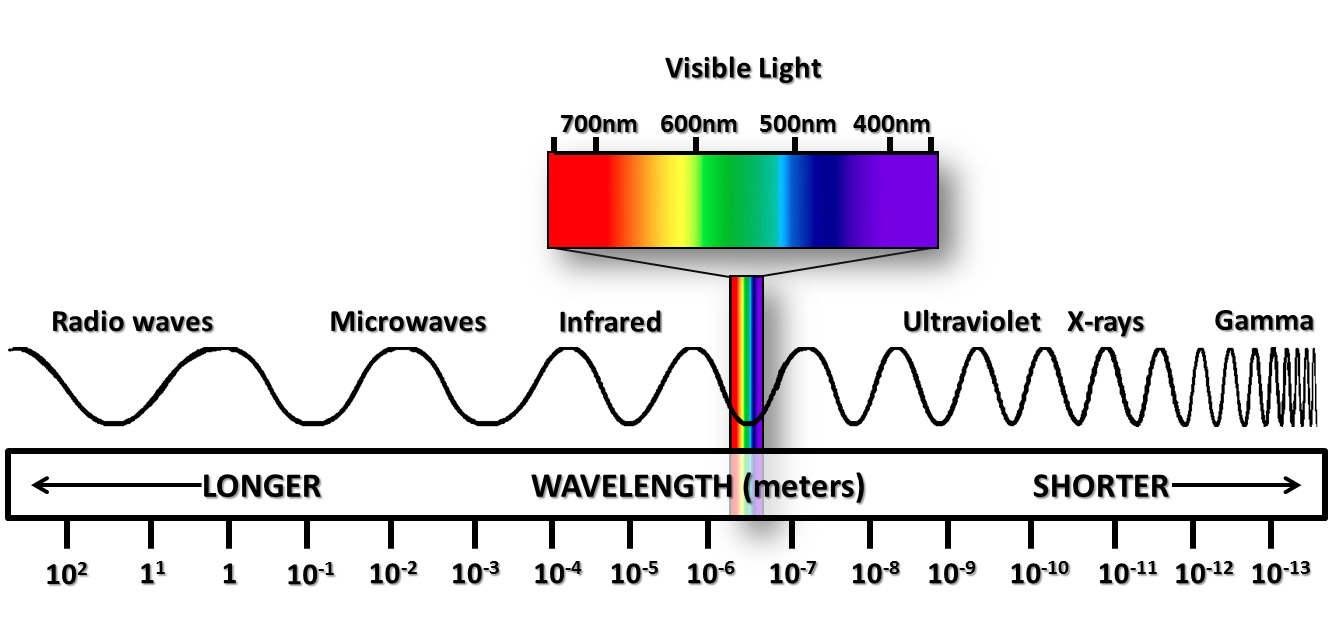
\includegraphics[width=0.75\textwidth]{figures/em_spectrum.png}
				\caption{Electromagnetic spectrum for reference.}
			\end{figure}
			\begin{enumerate}
				\item{Blackbody Radiation}
				\par Recall that the flux from an isotropically emitting surface is $F\propto T^4$, the Stefan-Boltzmann law. Furthermore, the Planck distribution function is given by,
				\begin{equation}
					B_{\nu}(T) = \frac{2h\nu^3/c^2}{e^{h\nu/kt} - 1}.
				\end{equation}
				Planck's function solved the ultraviolet catastrophe: namely, that the Rayleigh-Jean's law diverges for high frequencies. For $h\nu\gg kT$, the quantization of the photon must be taken into account. In a blackbody spectrum, we note that for a given $\lambda$, as $T$ increases, the intensity will also increase. Furthermore, as $T$ increases, the cutoff in $B_{\nu}$ moves to higher and higher $\lambda$.
				\item{Thermal versus Non-thermal}
				\par In general, we may regard thermal radiation as radiation emitted by matter in thermal equilibrium. Recall that the In the thermal case, we may assume that the velocity distribution of our particles is well-described by a Maxwellian, $dP\propto e^{-E/kT}d^3\mathbf{v}$. For non-thermal radiation, we may have radiation produced by particle populations who are not well-described by a Maxwellian. This may happen, for example, in accelerated electron beams in solar flares. 
				\item{Bremsstrahlung}
				\par Consider the case in which a free electron is elastically scattered by the Coulomb field of an ion and escapes as a free electron, a so-called \textit{free-free} transition. A photon is emitted with energy equal to the difference between the incoming and outgoing kinetic energy of the electron. This resulting emission is called \textit{bremsstrahlung}, or ``braking radiation''. For thermal bremsstrahlung, the spectral shape is $P_{\nu}\propto\exp{(-h\nu/kT)}$. X-ray bremsstrahlung generally arises from thermal plasmas though non-thermal bremsstrahlung can be observed in non-thermal electron beams in solar flares. The signature of bremsstrahlung is a smooth continuum with an exponential cutoff at $h\nu\sim kT$.
				\par Note that in the case of bremsstrahlung, the electrons are often assumed to be the radiators due to the fact that $\dot{v}\propto m^{-1}$. Recalling Larmor's formula,
				\begin{equation}
					P=\frac{2q^2\dot{u}^2}{3c^3},
				\end{equation}
				assuming $q_{ion}\approx q_{electron}$, we have that the power emitted by electrons is much greater than that emitted by the ions. 
				\par The bremsstrahlung emission due to a single particle can be written as 
				\begin{equation}
					\frac{dW}{d\omega dVdt} = \frac{16\pi e^2}{3\sqrt{3}c^3m^2v}n_en_iZ^2g_{ff}(v,\omega),
				\end{equation}
				where $g_{ff}$ is the Gaunt factor. To determine the Bremsstrahlung emission from a distribution of thermal particles, we can integrate this single-particle emissivity over a Maxwellian,
				\begin{equation}
					\frac{dW}{d\omega dV dt} = \frac{\int_{v_{min}}^{\infty}\frac{dW}{d\omega dt dV}v^2e^{-mv^2/2kt}\mathrm{d}v}{\int_0^{\infty}v^2e^{-mv^2/2kT}\mathrm{d}v}.
				\end{equation}
				The cutoff velocity, $v_{min}$, is due to the condition $h\nu\le mv^2/2$; essentially, the incoming particle must have at least as much energy as the outgoing photon. To find the bremsstrahlung emission due to nonthermal particles, we would need some sort of nonthermal spectrum (e.g. a power-law). We could then apply a similar treatment as we have done here in the thermal case. Note that non-thermal bremsstrahlung is particularly important in the production of hard x-rays in the flares. 
				%
				\item{Synchrotron}
				\par Particles accelerated by a magnetic field will radiate. In the event that these particles are nonrelativistic, they are said to emit cyclotron radiation at the cyclotron frequency. However, in the relativistic regime, the spectrum becomes more complex. This is synchrotron radiation. Synchrotron radiation refers to radiation emitted by any relativistic particle which is being accelerated perpendicular to its direction of motion (i.e. a circular path). 
				\par First, consider the relativistic Newton-Lorentz equations
				\begin{align}
					\frac{d}{dt}(\gamma m\mathbf{v}) = \frac{q}{c}\mathbf{v}\times\mathbf{B}, \\
					\frac{d}{dt}(\gamma mc^2)=q\mathbf{v}\cdot\mathbf{E}=0.
				\end{align}
				Separating out the components of $\mathbf{v}$ parallel and perpendicular to the field,
				\begin{align}
					\frac{d}{dt}\mathbf{v}_{\parallel} = 0,
					\frac{d}{dt}\mathbf{v}_{\perp} = \frac{q}{\gamma mc}\mathbf{v}_{\perp}\times\mathbf{B}.
				\end{align}
				The frequency of this motion is of course $\omega_B=qB/\gamma mc$. Using the Larmor formula for dipole radiation,
				\begin{equation}
					P=\frac{2q^2}{3c^3}\mathbf{a}\cdot\mathbf{a},
				\end{equation}
				the total emitted radiation for an isotropic velocity distribution is
				\begin{equation}
					P=\frac{4}{3}\sigma_Tc\beta^2\gamma^2U_B,
				\end{equation}
				where $\sigma_T=8\pi r_0^2/3$ is the Thomson scattering cross section and $U_B=B^2/8\pi$ is the magnetic energy density. Synchrotron emission becomes confined in a very narrow beam of width $2/\gamma$ directed perpendicular to to $\dot{v}$. Thus, as the motion becomes more relativistic, the emission becomes more strongly beamed. Synchrotron emission is particularly useful for measuring magnetic field strengths. 
			\end{enumerate}
			%
			\item{\em Observational Issues}
			\begin{enumerate}
				\item{Spectroscopy versus Imaging}
				\par \textbf{Imaging} instruments are sensitive to particular wavelength ranges such that within those ranges, they have no spectral resolution, meaning they cannot resolve individual spectral lines. These wavelength ranges are called channels. SDO/AIA is an example of a narrowband (relatively small ranges) while Hinode/XRT is an example of a broadband instrument. Channels are chosen to be centered on (or at least contain) particularly strong emission lines. Broad channels will cover a large spectral range, but consequently encapsulate many different emission lines. This creates ambiguity as to what you are actually looking at. For example, a channel centered on the 195\AA~ line of Fe XII ($1.6\times10^6$ K) may also contain a strong signal from the nearby Fe VII line ($0.6\times10^6$ K). Though their results are often ambiguous, imaging instruments have the advantage of multiple channels, wide fields of view, high cadence, and high spatial resolution. 
				\par Conversely, \textbf{spectrometers}, while sensitive to particular wavelength ranges, have spectral resolution within those wavelength ranges. Thus, they are able to resolve individual spectral lines, though line blending can still be an issue for nearby lines formed at similar temperatures. One of the biggest advantages of spectrometers is that you always know which line you are looking at. However, the trade-off comes in the form of both field-of-view and cadence. For example, Hinode/EIS, an imaging spectrometer, builds up an image by stepping the slit across the field-of-view. Thus, the field-of-view for a given step is only the width of the slit. Additionally, if the region-of-interest (ROI) changes significantly during the raster (which can take up to several hours), then there can be significant ambiguity in the results. Higher spatial resolution and cadence can be acheived, but this naturally results in lower photon counts and thus greater instrument noise. 
				%
				\item{Remote Sensing versus \textit{in-situ}}
				\par Essentially every solar observing instrument we use today is a \textbf{remote sensing} instrument. That is, it makes observations at a distance by gathering photons at given wavelengths, whether these are in channels (imaging instruments) or specific lines (spectrometers). Contrastingly, \textit{in-situ} detection would involve the direct measurement of coronal plasma (i.e. Van Allen probes in the radiation belts or MMS in the magnetotail), allowing for a completely unambiguous (or at least only up to instrument error) determination of particle energies. Currently, there are no operating \textit{in-situ} solar missions, though the Solar Probe Plus mission is currently scheduled for launch in 2018.
			\end{enumerate}
			%
			\item{\em Eruptive Phenomena}
			\begin{enumerate}
				\item{Flares}\\
				\citep[see][Ch. 10]{golub_solar_2010}
				%
				\par Flares, despite our proximity to the Sun and the wealth of observational data available, are difficult to study and classify. Flares emit an astounding amount of energy, $10^{33}$ erg on average, and are the most energetic events in the solar system. A flare can emit radiation from wavelengths $>10$ km in the radio to short wavelength x-rays and even gamma rays at $10^{-3}$ \AA~, spanning 17 orders of magnitude in wavelength. Flares are often classified by their total integrated soft x-ray output. This is determined, for example, by GOES, where each flare is assigned a ``class'' based on its peak intensity in the 1-8 \AA~ passband. This is shown in Table \ref{tab:goes_class}.
				%
				\begin{table}
					\centering
					\begin{tabular}{cc}
						\hline
						\hline
						Class & Intensity (erg cm$^{-2}$ s$^{-1}$) \\ \hline
						A$^{*}$ & weak \\
						B & $10^{-4}$ \\
						C & $10^{-3}$ \\
						M & $10^{-2}$ \\
						X & $10^{-1}$ \\ \hline\hline
					\end{tabular}
					\caption{\textit{GOES} flare classification \citep{golub_solar_2010}.}
					\label{tab:goes_class}
				\end{table}
				%
				\par While the theory behind flare evolution/production is still highly disputed, there is a general ``standard model'' of flare evolution which is as follows:
				\begin{enumerate}
					\item Magnetic free energy is stored in the corona, due either to motions of the photospheric footpoints or to the emergence of current-carrying field from below the photosphere. 
					\item A cool, dense filament forms, suspended by the magnetic field
					\item The field evolves slowly through equilibrium states, finally reaching a non-equilibrium (i.e. instability) which causes the closed field to rise. The field erupts outward into interplanetary space, ejecting chromospheric and/or coronal mass.
					\item The reconnection of the field below the rising arcade triggers the plasma heating and particle acceleration that we call the flare. Large H$\alpha$ structures, called ``post-flare loops,'' form over the polarity-inversion line via evaporation of chromospheric material.
				\end{enumerate}
				   
				%
				\item{Coronal Mass Ejections (CMEs)}
				
				%
				\item{Role of Reconnection}
				\par One of the major problems in flare modeling is to explain the rapid release of stored energy in the flare. The problem is the long diffusion time of magnetic fields in the corona, given by $\tau_d=L^2/\eta$, where $\eta$ is the resistivity. Typically, $\tau_d\sim10^{10}-10^{16}$ s,m far too slow for flare energy release timescales. The most promising solution to this problem is of course \textit{magnetic reconnection}. Using the simple Sweet-Parker neutral sheet picture, we can easily find that the inflow velocity is $v=v_A/\sqrt{R_m}$, where $v_A\equiv B/\sqrt{4\pi\rho}$ is the Alfv\'en velocity and $R_m$ is the magnetic Reynolds number, the ratio of the diffusion to the advection time. In the Sweet-Parker picture, these timescales are still too long; the Petschek picture improves on this by making the diffusion region smaller and noting that MHD waves can accelerate the field into the diffusion region, thereby lowering the diffusion time. However, the timescales predicted by these models are still too long to explain observed flares. 
			\end{enumerate}
			%
			\item{\em Solar Wind}
			\par Coronal loops are magnetically closed regions in which no particles can esacpe. However, there are also magnetically \textit{open} regions which can provide a way for particles to escape from the Sun. One example of an open region is a \textit{coronal hole}, one proposed path for particles escaping to create the \textit{solar wind}. \citet{biermann_kometenschweife_1951} first suggested that comet tail orientations required an outflow of gas from the Sun with a velocity $500\le v\le 1500$ km s$^{-1}$. Measurments of the solar wind by \textit{Mariner II} and \textit{Ulysses} later confirmed the existence of this wind
			%
			\begin{enumerate}
				\item{Fast versus Slow Wind}
				\par The slow solar wind originates from regions closer to the equator (farther from the poles) and produce a solar wind of approximately 400 km s$^{-1}$. The slow wind is usually said to originate in closed-field regions where the dominant energy loss mechanism is downward thermal conduction. 
				%
				\par The fast solar wind originates from the more abundant open field regions near the poles. These carry the solar wind out at a speed of approximately 800 km s$^{-1}$. Here, the dominant loss mechanisms are due to work done against gravity and the kinetic energy of the flow. Additionally, some heating is needed farther out in the wind (e.g. Alfv\'en wave dissipation) in order to obtain ``fast'' speeds. Additionally, higher temperatures have been observed for ions than for electrons, supporting the idea of some preferential energy deposition mechanism.
				%
				\item{Parker Spiral}
				%
				\par The expanding outflow of material from the Sun has a significant effect on the interplanetary magnetic field. Because the interplanetary magnetic field is ``frozen-in'', the field moves with plasma such that as material flows out in the solar wind, a given magnetic field line is draw along the path of the fluid element. We consider the simple case of spherical expansion.
				\par We first consider the case of simple radial expansion where the Sun is not rotating. We invoke magnetic flux conservation such that 
				\begin{equation}
					\Phi\equiv\int\mathrm{d}\mathbf{S}\cdot\mathbf{B},
				\end{equation}
				is invariant over $r$. Thus, we can write,
				\begin{equation}
					\Phi(r_0)=\int\mathrm{d}\mathbf{S}\cdot B_0\hat{r} = B_0r_0^2\int\mathrm{d}\phi\int\mathrm{d}\theta\sin{(\theta)} = B_rr^2\int\mathrm{d}\phi\int\mathrm{d}\theta\sin{(\theta)} = \Phi(r),
				\end{equation}
				such that the radial component of the field can be written as,
				\begin{equation}
					B_r = B_0\left(\frac{r_0}{r}\right)^2.
				\end{equation}
				We can derive the azimuthal component of the field by a similar argument. An area element at the surface of the Sun $\mathrm{d}\mathbf{A}_0=\mathrm{d}A_0\hat{r}$ has area $\mathrm{d}A_0=r_0^2\mathrm{d}\phi\sin{(\theta)}\mathrm{d}\theta$. An element oriented in the azimuthal direction (at $\infty$ along the spiral) $\mathrm{d}\mathbf{A}_{\infty}=\mathrm{d}A_{\infty}\hat{\phi}$ has area $\mathrm{d}A_{\infty} = \mathrm{d}r(r\mathrm{d}\theta)$. Again, using flux conservation,
				\begin{align}
					\mathbf{B}_{\phi}\cdot\mathrm{d}\mathbf{A} &= \mathbf{B}_0\cdot\mathrm{d}\mathbf{A}, \\
					B_{\phi}r\mathrm{d}r\mathrm{d}\theta &= B_0r_0^2\sin{(\theta)}\mathrm{d}\theta\mathrm{d}\phi, \\
					B_{\phi} &= B_0\frac{r_0^2}{r}\frac{\mathrm{d}\phi}{\mathrm{d}r},
				\end{align}
				where $\sin{(\theta)}=1$ because we are evaluating our expression in the equatorial plane. Noting that $\mathrm{d}r/\mathrm{d}t=v_{sw}$ is the velocity of the solar wind and $\Omega=-\mathrm{d}\phi/\mathrm{d}t$, we can write,
				\begin{equation}
					B_{\phi} = -\frac{B_0\Omega}{v_{sw}}\frac{r_0^2}{r}.
				\end{equation}
				We see that $B_{\phi}\propto r^{-1}$ while $B_r\propto r^{-2}$ such that as $r\to\infty$, $B_\phi$ dominates over $B_r$. Note also that integrating $\mathrm{d}r/\mathrm{d}\phi=-v_{sw}/\Omega$ yields,
				\begin{equation}
					r - r_0 = -\frac{v_{sw}}{\Omega}(\phi - \phi_0),
				\end{equation}
				showing that the field lines trace out a spiral as they expand radially.
				%
				\item{Parker's Model}
				\par In an effort to show the inevitability of the solar wind, \citet{parker_dynamics_1958} showed through simple hydrodynamics (i.e. without considering the magnetic field) that the pressure of the interstellar/interplanetary medium was far too small to support a corona in hydrostatic equilibrium at these distances such that expansion (i.e. the solar wind) is inevitable. 
				\par We start with our set of hydrodynamic equations,
				\begin{align}
					\frac{\partial p}{\partial r} + \frac{GM_{\odot}Mn}{r^2} = 0, \\
					E_H - \nabla\cdot(-\kappa(T)\nabla T) - E_R = 0,
				\end{align}
				along with the closure condition $p=2nk_BT$. The thermal conductivity coefficient is expressed as $\kappa(T) = \kappa_0T^n$. We first want to derive an expression for the temperature. We note that far enough out in the wind $E_H,E_R\to 0$. Additionally, we will use spherical coordinates such that the energy equation becomes,
				\begin{align}
					-\nabla\cdot(\kappa(T)\nabla T) = 0, \\
					-\frac{1}{r^2}\frac{\partial}{\partial r}\left(-r^2\kappa_0T^n\frac{\partial T}{\partial r}\right) = 0, \\
					-r^2\kappa_0T^n\frac{\partial T}{\partial r} = C_1,
				\end{align}
				where $C_1$ is a constant. We can very easily perform a separation of variables on this differential equation,
				\begin{equation}
					\int^T_{T_a}\mathrm{d}T~T^n = -\frac{C_1}{\kappa_0}\int^r_a\mathrm{d}r~r^{-2},
				\end{equation}
				where $r=a$ corresponds to the corona. Defining $\lambda\equiv C_1(n+1)/\kappa_0T_a^{n+1}$, the radial temperature profile can be written,
				\begin{equation}
					T(r)=T_a\left(1+\lambda\left(\frac{1}{r} - \frac{1}{a}\right)\right).
				\end{equation}
				\par To find an equation for the pressure, we consider the pressure balance equation
				\begin{equation}
					\frac{\partial (nT)}{\partial r} = -\frac{GM_{\odot}M}{2k_B}\frac{n}{r^2}.
				\end{equation}
				Separating variables, using the chain rule, and dividing both sides by $nT$, we have
				\begin{equation}
					\int_{n_a}^{n}\mathrm{d}n'~\frac{1}{n'} + \int_{T_a}^{T}\mathrm{d}T'~\frac{1}{T'} = -\frac{GM_{\odot}M}{2k_B}\int^r_a\mathrm{d}r~\frac{1}{T(r)r^2}.
				\end{equation}
				Using the radial temperature profile we derived above, defining $\Lambda\equiv GM_{\odot}M/2k_B\lambda T_a$, and making a change of variables $\psi\equiv 1 + \lambda(1/r - 1/a)$, 
				\begin{equation}
					\ln{\frac{nT}{nT_a}} = \Lambda\int^{\psi}_{\psi_a}\mathrm{d}\psi'~\psi'^{-\frac{1}{n+1}}.
				\end{equation}
				Noting that $\psi_a=1$ and $\ln{nT/nT_a}=\ln{p/p_a}$ this expression can be easily integrated to find
				\begin{equation}
					p(r) = p_a\exp\left(\Lambda\frac{n+1}{n}\left(\left(1 + \lambda\left(\frac{1}{r} - \frac{1}{a}\right)\right)^{n/n+1} - 1 \right)\right).
				\end{equation}
				We want to find $p(r\to\infty)$. Looking back to our radial temperature profile, we can use some algebra to find
				\begin{equation}
					\left(\frac{T}{T_a}\right)^{n+1} - 1 = \lambda\left(\frac{1}{r} - \frac{1}{a}\right).
				\end{equation}
				As $r\to\infty$, $T$ falls off such that $T(\infty)/T(a)\ll1$, exacerbated by larger $n$. Thus, from the above expression, we find that $\lambda\approx a$. Plugging this into our expression for $p(r)$ at $r\to\infty$, we find that 
				\begin{equation}
					p_{\infty} = p_a\exp\left(-\Lambda\frac{n+1}{n}\right).
				\end{equation}
				Using typical values of $T_a,n_a$ at $r=a=10^{11}$ cm, for $n=1/2$, $p_{\infty}\approx1.2\times10^{-9}$ dyne cm$^{-2}$ and for $n=5/2$, $p_{\infty}=6.6\times10^{-6}$ dyne cm$^{-2}$. Observations indicate that the interstellar pressure is $p_{\infty}\approx1.4\times10^{-13}$, many orders of magnitude less than that predicted by a hydrostatic approach! Thus, we can conclude that it is not possible for the corona to be confined in hydrostatic equilibrium out to large distances and thus we expect some outward hydrodynamic expansion of the coronal gas.
				%
				\par To take into account steady expansion of the corona, we reconsider our pressure (momentum) equation and do not neglect terms involving the velocity. We also take into consideration the mass continuity equation,
				\begin{align}
					nM\frac{\partial v}{\partial r} =& -\frac{\partial(2nk_BT)}{\partial r} - \frac{GMM_{\odot}n}{r^2}, \\
					\frac{\partial(r^2nv)}{\partial r} =& 0.
				\end{align}
				From the mass continuity equation, we find that $r^2nv=\text{const}$. Thus, 
				\begin{equation}
					nv = n_av_a\left(\frac{a}{r}\right)^2.
				\end{equation}
				Substituting this expression into the momentum equation to eliminate $n$ and using the dimensionless variables
				\begin{equation}
					\xi\equiv\frac{r}{a},\quad\tau\equiv\frac{T}{T_a},\quad\lambda\equiv\frac{GM_{\odot}M}{2k_BT_aa},\quad\psi\equiv\frac{Mv^2}{2k_BT_a},
				\end{equation}
				and a lot of algebra, we can derive the dimensionless differential equation,
				\begin{equation}
					\left(1 - \frac{\tau}{\psi}\right)\frac{\partial\psi}{\partial\xi} = -2\xi^2\frac{\partial}{\partial\xi}\left(\frac{\tau}{\xi^2}\right) - \frac{2\lambda}{\xi^2}.
				\end{equation}
				In order to integrate this equation, we say that for $a<r\le b$, coronal heating maintains a constant temperature of $T_a$ and $\tau=1$. For $r>b$, the heating vanishes and $T\ll T_a$ such that $\tau=0$. Thus, for all three ($r<b,~r=b,~r>b$) of these cases, we find that
				\begin{align}
					\psi - \ln{\psi} &= \psi_a - \ln{\psi_a} + 4\ln{\xi} - 2\lambda\left(1-\frac{1}{\xi}\right),&\quad r<b, \\
					\psi &= \psi_b,&\quad r=b, \\
					\psi &= \psi_b - 2\lambda(\frac{a}{b} - \frac{1}{\xi}),&\quad r>b.
				\end{align}
				We want to know whether a subsonic wind at $r=a$ can produce the supersonic wind that we observe near Earth ($r=b$). Because we demand that $v\in\mathbb{R}$, we want only solutions where $\psi\propto v^2 >0$. Thus, we look at solutions where $r<b$. Noting that the LHS is minimized when $\psi=1$ and the RHS is minimized when $\xi=\lambda/2$, and requiring that these minima occur simultaneously, we can derive an expression for $\psi_a-\ln{\psi_a}$, allowing us to graphically determine a solution for $\psi$. \citet{parker_dynamics_1958} found that a 500 km s$^{-1}$ outflow arises at $r=200a$ when $T_a=10^6$ K. Thus, thermal speeds for coronal temperatures are able to accelerate coronal gas to the observed solar wind speeds and allow the gas to escape the solar gravitational field. 
				%
			\end{enumerate}
		\end{enumerate}